\documentclass[aspectratio=169]{beamer}
\usepackage{amsmath}
\usepackage{graphicx}
\usepackage{caption}
\usepackage{siunitx}
\usepackage{mhchem}
\usepackage{subcaption}
\usepackage{appendixnumberbeamer}
\usetheme{AnnArbor}
\usecolortheme{whale}
\title{Performance evaluation of the 8-inch MCP-PMT}
\author{Zhang Aiqiang}
\institute{Tsinghua University}
\date{2022/12/22}
\begin{document}
\begin{frame}[noframenumbering]
    \titlepage
\end{frame}
\begin{frame}[noframenumbering]
    \tableofcontents
\end{frame}
\section{Introduction}
\begin{frame}{Introduction}
    \begin{columns}
        \begin{column}{0.4\textwidth}
            \begin{figure}
                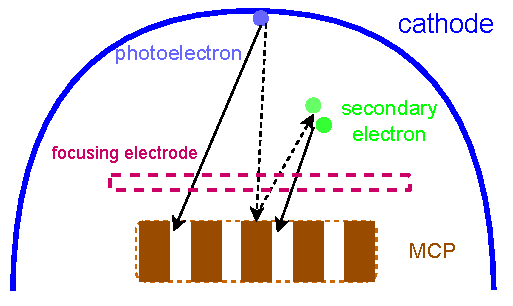
\includegraphics[width=\columnwidth]{../figures/method/MCPelectron.pdf}
            \end{figure}
        \end{column}
        \begin{column}{0.6\textwidth}
            \begin{enumerate}
                \item PMT transforms a photon to the measurable signal
                \item MCP-PMT multipy photoelectron inside MCP
                \item Jinping Neutrino Experiment plan to use the 8-inch MCP-PMT from NNVT
            \end{enumerate}
        \end{column}
    \end{columns}
    \begin{block}{Requirement}
        \begin{enumerate}
            \item Good cost performance
            \item High photon detection efficiency (PDE)
            \item Transit Time Spread (TTS): ns scale
        \end{enumerate}
    \end{block}
\end{frame}

\section{Experimental setup and test procedures}
\begin{frame}{Experimental setup}
    \begin{columns}
        \begin{column}{0.4\textwidth}
            \begin{figure}
                \includegraphics[width=\columnwidth]{../figures/facility/schema.pdf}
            \end{figure}
        \end{column}
        \begin{column}{0.6\textwidth}
            \begin{enumerate}
                \item CAEN V1751 ditizer: 10-bit, \SI{1}{GHz} (1 quantisation level is denoted as 1ADC)
                \item Wiener EDS 30330p high voltage
                \item PiL040XSM laser: picosecond, \SI{405}{nm}, trigger signal output
                \item The digitizer, HV, and laser are controlled by custom-made DAQ software
            \end{enumerate}
        \end{column}
    \end{columns}
    \begin{enumerate}
        \item Dark room: black plastic box, split into 4 grids
        \item Fiber splitter: 1 to 4 channels, each port covered with \SI{4}{cm\tothe{2}} square diffuser plate
        \item 9 MCP-PMTs and 1 reference dynode PMT are tested
    \end{enumerate}
\end{frame}

\begin{frame}{Test procedures}
    \begin{columns}
        \begin{column}{0.4\textwidth}
            \begin{figure}
                \includegraphics[width=\columnwidth]{../figures/facility/procedure.pdf}
            \end{figure}
        \end{column}
        \begin{column}{0.6\textwidth}
            \begin{itemize}
                \item HV: provided by vendor
                \item Cooling down: at least 12h
                \item Meta data: PMT-box map
                \item Automation
            \end{itemize}
        \end{column}
    \end{columns}
\end{frame}
\section{Characterization method and results}
\subsection{preanalysis}
\begin{frame}{preanalysis}
    \begin{columns}
        \begin{column}{0.45\textwidth}
            \begin{figure}
                \includegraphics[width=\columnwidth]{../figures/method/triggerwave.pdf}
                \includegraphics[width=\columnwidth]{../figures/method/noisebaseline697_219908_2.pdf}
            \end{figure}
        \end{column}
        \begin{column}{0.55\textwidth}
            \begin{itemize}
                \item Sample window size $T_{\mathrm{wave}}$: \SI{10400}{ns}
                \item The rising edge of trigger waveform: about \SI{200}{ns}
                \item Trigger time $t_{\mathrm{trig}}$: linearly interpolated
                \item Preanalysis window $[t_{\mathrm{trig}},T_{\mathrm{wave}}]$ ($600\mathrm{ns}$)
            \end{itemize}

            \begin{itemize}
                \item The maximum pulse. The peak time $t_p$. The peak height $V_p$
                \item Baseline: threshold filter
            \end{itemize}
        \end{column}
    \end{columns}
\end{frame}
\begin{frame}{preanalysis}
    \begin{columns}
        \begin{column}{0.6\textwidth}
            \begin{figure}
                \includegraphics[width=\columnwidth]{../figures/method/triggerwave.pdf}
            \end{figure}
        \end{column}
        \begin{column}{0.4\textwidth}
            \begin{figure}
                \includegraphics[width=\columnwidth]{../figures/method/triggerpeakpos.pdf}
            \end{figure}
        \end{column}
    \end{columns}
    \begin{itemize}
        \item G$(\mu_{t0},\sigma_{t0})$ is unbinned fitted to the distribution of $t_p-t_{\mathrm{trig}}$ of pulses
        \item Candidate window: $[\mu_{t0}-5\sigma_{t0}, \mu_{t0}+5\sigma_{t0}]$
    \end{itemize}
\end{frame}
\subsection{Peak and charge spectrum}
\begin{frame}{Peak and charge spectrum}
    \begin{columns}
        \begin{column}{0.4\textwidth}
            \begin{figure}
                \includegraphics[width=\columnwidth]{../figures/method/triggercharge.pdf}    
            \end{figure}
        \end{column}
        \begin{column}{0.4\textwidth}
            \begin{figure}
                \includegraphics[width=\columnwidth]{../figures/method/triggerpeak.pdf}
            \end{figure}
        \end{column}
    \end{columns}
    \begin{itemize}
        \item $C_{\mathrm{equ}}$: $[-15, 75]$\,ns relative to $t_p$
        \item Peak: G$(C_1,\sigma^2_{C_1})$, binned fit $[0.65C_1, 1.35C_1]$
        \item Vally: A parabolic function,$[-0.15C_1, 0.25C_1]$
        \item Mean $\mu_{C}$ and sample variance $s^2_{C}$ of $C_{\mathrm{equ}}$: $V_p$ higher than \SI{3}{ADC} and $C_{\mathrm{equ}}$ larger than 0.25$C_1$
    \end{itemize}
\end{frame}
\begin{frame}{Gain and single PE resolution}
    \begin{columns}
        \begin{column}{0.38\textwidth}
            \begin{figure}
                \includegraphics[width=\columnwidth]{../figures/result/gainres.pdf}    
            \end{figure}
        \end{column}
        \begin{column}{0.6\textwidth}
            \begin{itemize}
                \item The gain of the main peak $G_1$: $\frac{C_1}{e\times 50\Omega}$
                \item The gain of the total charge $G$: $G\frac{\mu_{C}}{e\times 50\Omega}$
                \item The main peak resolution $\mathrm{Res}_1$: $\frac{\sigma_{C_1}}{C_1}$
                \item The total charge resolution$\mathrm{Res}$: $G\frac{\mu_{C}}{e\times 50\Omega}$
            \end{itemize}

            \begin{itemize}
                \item $G$ is about 2 times $G_1$ for the MCP-PMTs
                \item Mean of $\mathrm{Res}_1$, $\mathrm{Res}$: about 0.25, 0.69
            \end{itemize}
        \end{column}
    \end{columns}
    \begin{block}{Peak-to-valley ratio and some time characteristics}
        \begin{enumerate}
            \item The mean P/V ratio of MCP-PMTs is about 5.8 while the reference PMT is about 2.4.
            \item Estimated mean and deviation of rise time, fall time, and FWHM are $3.71\pm0.15$\,ns, $15.6\pm1.8$\,ns, and $9.07\pm0.63$\,ns for 9 MCP-PMTs.
        \end{enumerate}
    \end{block}
\end{frame}
\subsection{TTS}
\begin{frame}{TT}
    \begin{columns}
        \begin{column}{0.7\textwidth}
            \begin{figure}
                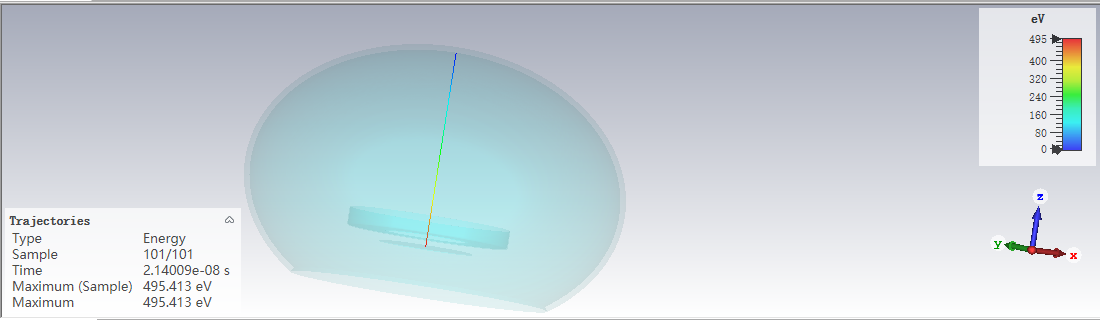
\includegraphics[width=\columnwidth]{driftTime.png}
            \end{figure}
        \end{column}
        \begin{column}{0.3\textwidth}
            \begin{itemize}
                \item Cathode, focus dynode, MCP
                \item CST studio: electric field and trajectory simulation
            \end{itemize}
        \end{column}
    \end{columns}
    \begin{columns}
        \begin{column}{0.4\textwidth}
            \begin{figure}
                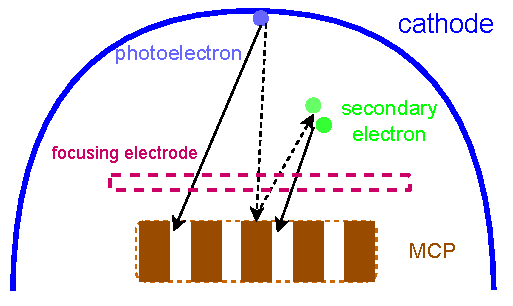
\includegraphics[width=\columnwidth]{../figures/method/MCPelectron.pdf}    
            \end{figure}
        \end{column}
        \begin{column}{0.6\textwidth}
            \begin{itemize}
                \item The drift times of the electrons at the top of PMT with \SI{0}{eV} and \SI{3}{eV} are respectively about \SI{21}{ns} and \SI{18}{ns}
                \item The electrons hitting on the surface of MCP generate the secondary electrons (including a single elastic scattering electron)
            \end{itemize}
        \end{column}
    \end{columns}
\end{frame}
\begin{frame}{TTS}
    \begin{columns}
        \begin{column}{0.33\textwidth}
            \begin{figure}
                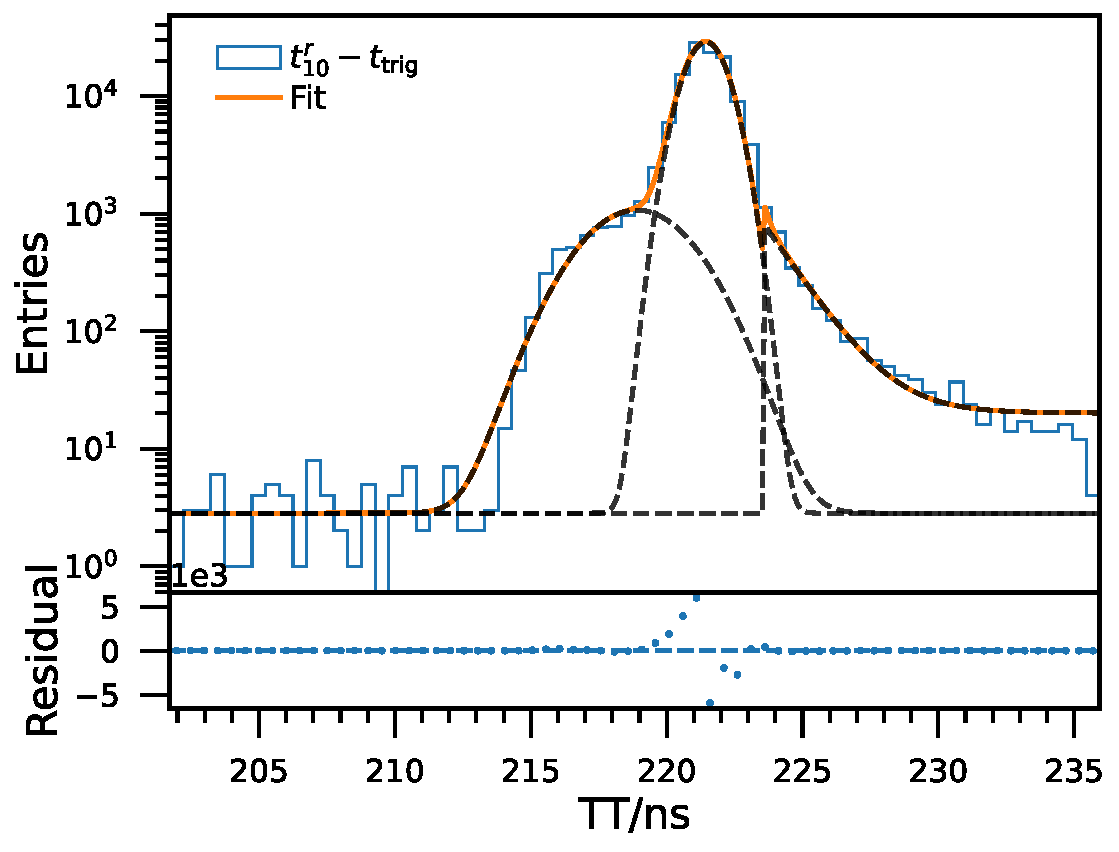
\includegraphics[width=\columnwidth]{../figures/method/triggerTTSLog.pdf}    
            \end{figure}
        \end{column}
        \begin{column}{0.33\textwidth}
            \begin{figure}
                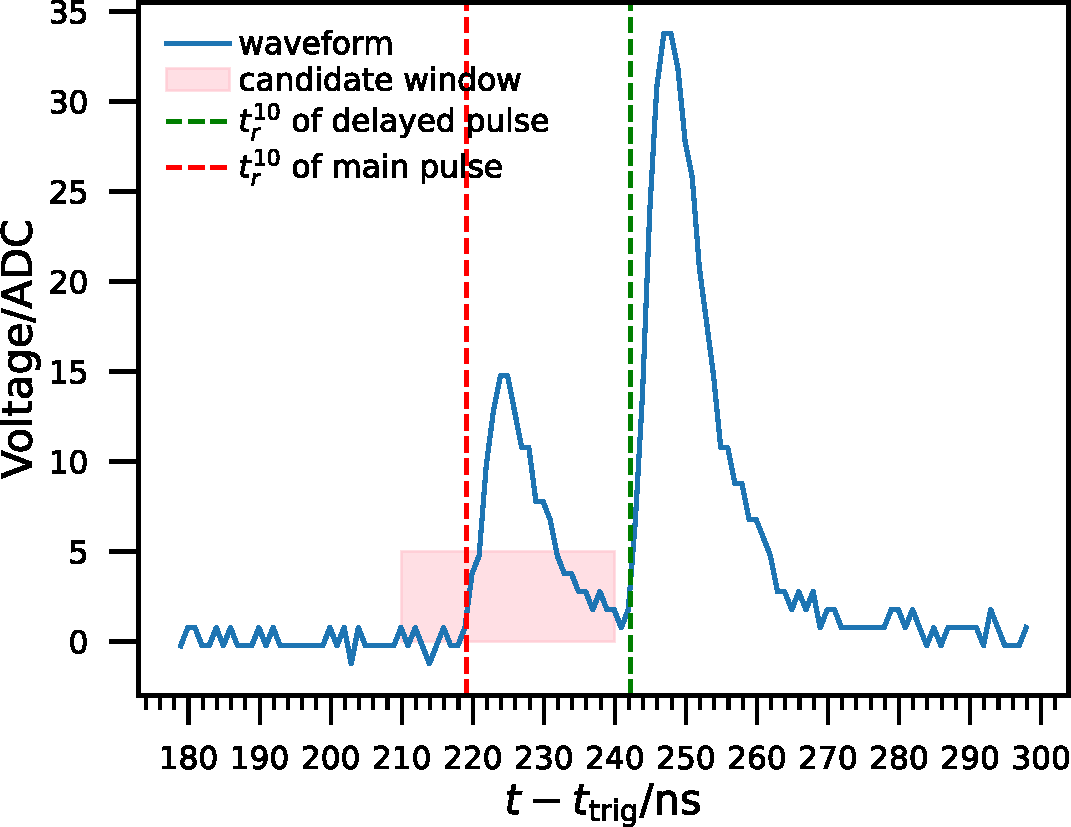
\includegraphics[width=\columnwidth]{../figures/method/triggerDoublePulse.pdf}    
            \end{figure}
        \end{column}
        \begin{column}{0.33\textwidth}
            \begin{figure}
                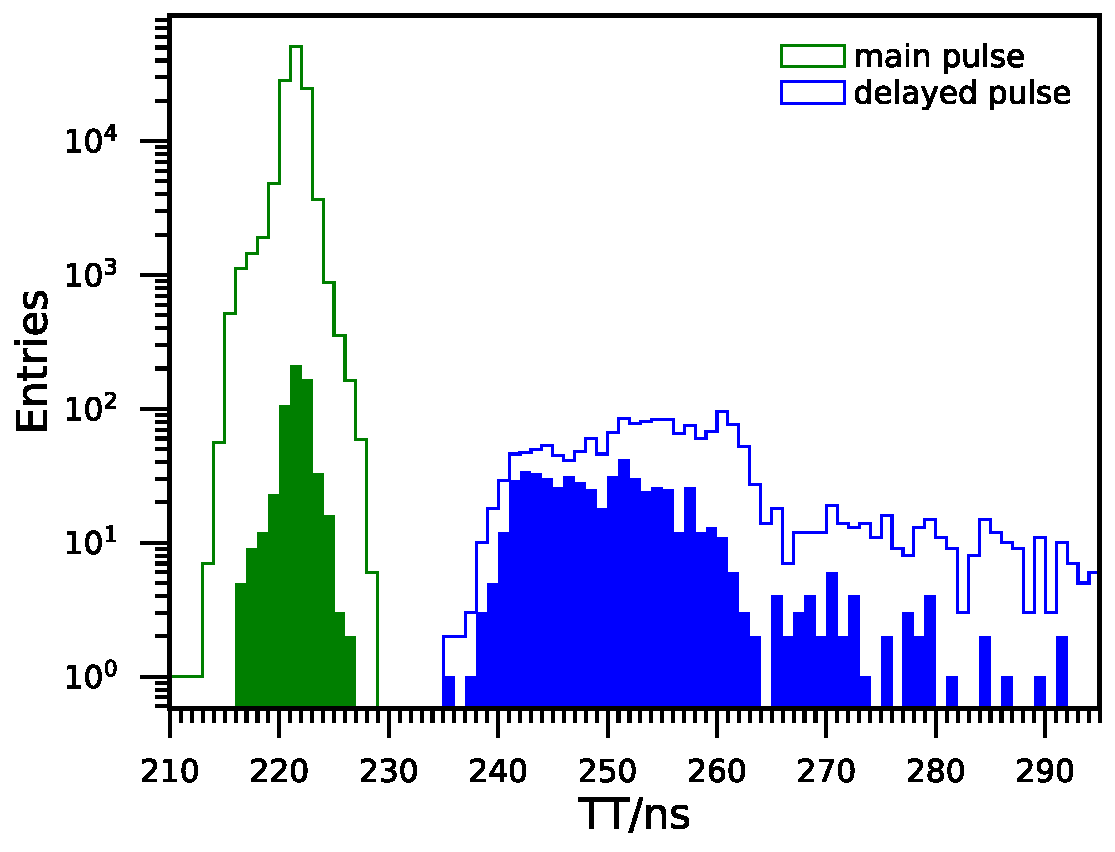
\includegraphics[width=\columnwidth]{../figures/method/triggerDelayedPulse.pdf}    
            \end{figure}
        \end{column}
    \end{columns}
    \begin{itemize}
        \item Multiple secondary electrons with different kinetic energy may cause two or more pulses
        \item Elastic scattering electrons: The sharp difference between them at about \SI{40}{ns} after the main peak, twice times drift time of electrons from the cathode to the MCP
        \item $B+N_tG(\mu_{\mathrm{TT}},\sigma_{\mathrm{TT}}^2)+N_KG(\mu_K,\sigma_K^2)+H(\mu_{\mathrm{TT}}+2\sigma_{\mathrm{TT}})\left(b_S+N_Se^{-\frac{t-(\mu_{\mathrm{TT}}+2\sigma_{\mathrm{TT}})}{\tau_S}}\right)$
    \end{itemize}
\end{frame}
\begin{frame}{TTS}
    \begin{columns}
        \begin{column}{0.33\textwidth}
            \begin{figure}
                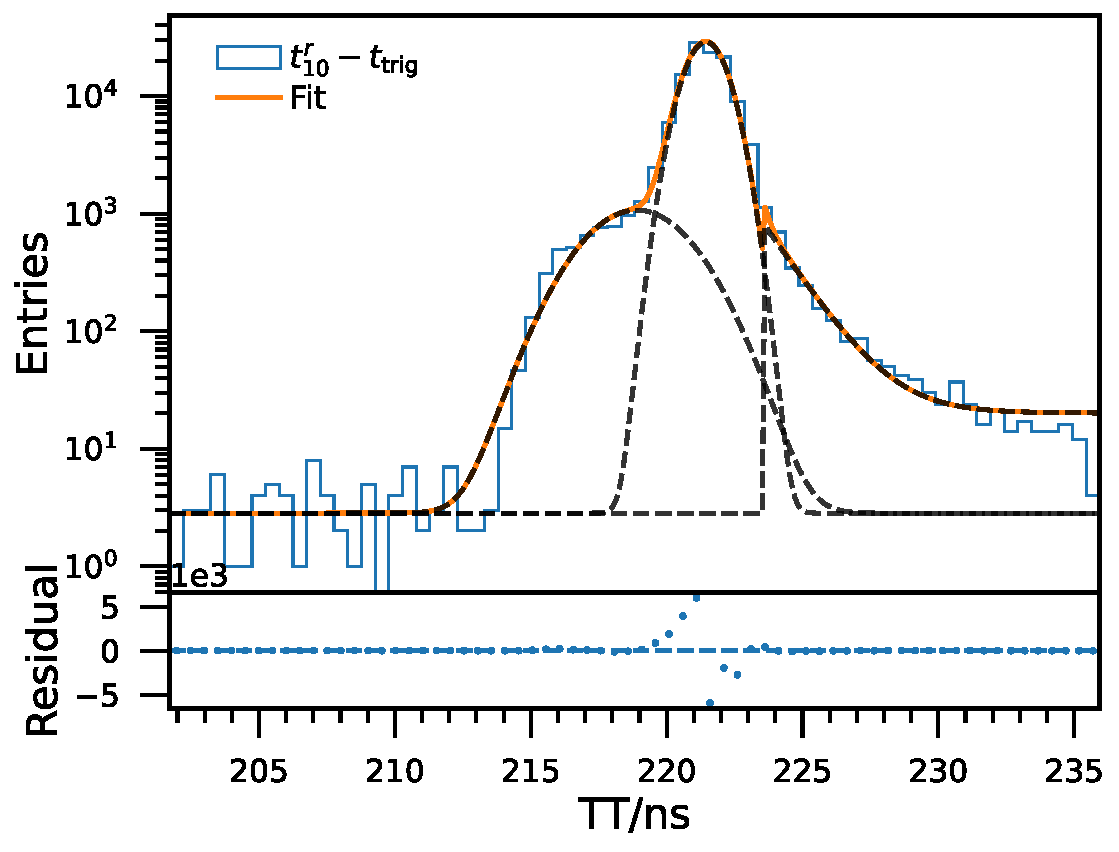
\includegraphics[width=\columnwidth]{../figures/method/triggerTTSLog.pdf}    
            \end{figure}
        \end{column}
        \begin{column}{0.33\textwidth}
            \begin{figure}
                \includegraphics[width=\columnwidth]{../figures/method/triggerTTS.pdf}    
            \end{figure}
        \end{column}
        \begin{column}{0.33\textwidth}
            \begin{figure}
                \includegraphics[width=\columnwidth]{../figures/method/triggerTTS2d.pdf}    
            \end{figure}
        \end{column}
    \end{columns}
    \begin{itemize}
        \item TTS is defined as FWHM: $2\sqrt{2\ln(2)}\sigma_{\mathrm{TT}}$
        \item The long tail in charge distribution
    \end{itemize}
\end{frame}
% \subsection{Single electron response}
% \begin{frame}{Single electron response}
%     \begin{columns}
%         \begin{column}{0.33\textwidth}
%             \begin{figure}
%                 \includegraphics[width=\columnwidth]{../figures/method/triggerSER.pdf}
%             \end{figure}
%         \end{column}
%         \begin{column}{0.33\textwidth}
%             \includegraphics[width=\columnwidth]{../figures/method/triggerSER2d.pdf}
%         \end{column}
%         \begin{column}{0.33\textwidth}
%             \includegraphics[width=\columnwidth]{../figures/result/tausigma.pdf}
%         \end{column}
%     \end{columns}
%     \begin{itemize}
%         \item The FWHM of candidate pulses : \SI{2}{ns}-\SI{15}{ns}
%         \item A charge filter $[0.5C_1, 1000\mathrm{ADC\cdot ns}]$
%     \end{itemize}
% \end{frame}
\subsection{Pre-pulse and after-pulse}
\begin{frame}{After pulse categories}
    \begin{columns}
        \begin{column}{0.45\textwidth}
            \begin{figure}
                \includegraphics[width=\columnwidth]{../figures/method/triggerAfterpulseSchema.pdf}
                \includegraphics[width=\columnwidth]{../figures/method/triggerAfterpulse1d.pdf}
            \end{figure}
        \end{column}
        \begin{column}{0.55\textwidth}
            \begin{itemize}
                \item Pre-pulses: photons hitting on the MCP or the first dynode directly rather than the photocathode; \SI{10}{ns} scale
                \item After-pulses: the ionization of gaseous impurities between the cathode and first dynode or MCP when photoelectrons go through;\SI{100}{ns} scale
                \item After-pulses: the relation between time and ions (\ce{^Z_MX}) is $\sqrt{\frac{M}{Z}}$
                \item Search window: $<$\SI{-10}{ns}; $>$\SI{200}{ns}
                \item The peak position $t_p$ and equivalent charge $C_{\mathrm{equ}}$ of the after-pulse and pre-pulse are calculated
            \end{itemize}
        \end{column}
    \end{columns}
\end{frame}
\begin{frame}{Parameterization}
    \begin{columns}
        \begin{column}{0.45\textwidth}
            \begin{figure}
                \includegraphics[width=\columnwidth]{../figures/method/triggerAfterpulse1d.pdf}
                \includegraphics[width=\columnwidth]{../figures/method/triggerAfterpulse2d.pdf}
            \end{figure}
        \end{column}
        \begin{column}{0.55\textwidth}
            \begin{itemize}
                \item The relative t: the difference between $t_p$ of pre/after-pulse and $t_r^{10}$ of main pulse
                \item around \SI{300}{ns}, \SI{550}{ns}, \SI{1200}{ns} and \SI{1700}{ns}, $1:\sqrt{3}:\sqrt{16}:\sqrt{32}$
                \item Assumption: \ce{H^+}, \ce{He^{+}} or other unknown ions, \ce{O^+} or \ce{CH_4^+}, and \ce{O_2^+} or other unknown ions
                \item Substracting dark noise rate $N_{\mathrm{DCR}}=N_{\mathrm{trig}}\cdot \mathrm{DCR}\cdot T_{\mathrm{bin}}$, in which $N_{\mathrm{trig}}$ is the number of triggered waveforms
                \item $\sum_{i=1}^{4}{A_iG(t_i,\sigma_i^2)}$
                \item $[-150,-10]$\,ns $[200,9800]$\,ns
            \end{itemize}
        \end{column}
    \end{columns}
\end{frame}

\begin{frame}{Dark count rate}
    \begin{equation}
        \mathrm{DCR/kHz} = \frac{N_{\mathrm{noise}}}{N_{\mathrm{trig}}}\frac{1}{T_{\mathrm{DCR}}/\mathrm{ns}}\times 10^{6}
    \end{equation}
    \begin{itemize}
        \item $[-200,-150]$\ ns relative to main pulse
        \item $T_{\mathrm{DCR}}$ is \SI{50}{ns}
    \end{itemize}
\end{frame}
\subsection{Relative PDE}
\begin{frame}{Relative PDE}
    \begin{enumerate}
        \item total light intensity  $I_n$ for nth run, jth splitter ratio $\alpha_j$, kth PMT PDE $\eta_k$
        \item Expected photon number $p_{njk}=I_n\alpha_j\eta_k$
        \item Observed trigger rate $R_{njk}=1-e^{-p_{njk}}$
    \end{enumerate}
    0th PMT is the only one reference PMT. $\alpha_j^0=\frac{\alpha_j}{\alpha_0}$, $\eta_k^0=\frac{\eta_k}{\eta_0}$, $I_n^0=I_n\alpha_0\eta_0$, $i\equiv njk$
    \begin{equation}
        \label{equ:pdelograte}
        \mathrm{log}(p_{i})=\mathrm{log}(I_0\alpha_0\eta_0)+\mathrm{log}(I_n^0)+\mathrm{log}(\alpha_j^0)+\mathrm{log}(\eta_k^0)
    \end{equation}

    \begin{equation}
        \label{equ:linkfunction}
        R_{i}=1-e^{-e^{\mathrm{log}(I_0\alpha_0\eta_0)+\mathrm{log}(I_n^0)+\mathrm{log}(\alpha_j^0)+\mathrm{log}(\eta_k^0)}}
    \end{equation}
    The trigger number $N_{{\mathrm{trig}_{i}}}$ of kth PMT in nth run with jth splitter obey Binomial distribution $B(R_{i},N_{t_{i}})$, in which $N_{t_{i}}$ is total number of waveforms.

    \begin{equation}
        \label{equ:likelihood}
        \mathcal{L}=\prod_{i}{R_{i}^{N_{\mathrm{trig}_{i}}}(1-R_{i})^{N_{t_{i}}-N_{\mathrm{trig}_{i}}}}
    \end{equation}
General linear model of Binomial exponential family distribution with Cloglog link function
\end{frame}
\section{Energy resolution boost}
\begin{frame}{Energy resolution boost}
    \begin{columns}
        \begin{column}{0.4\textwidth}
            \begin{figure}[!htbp]
                \centering
                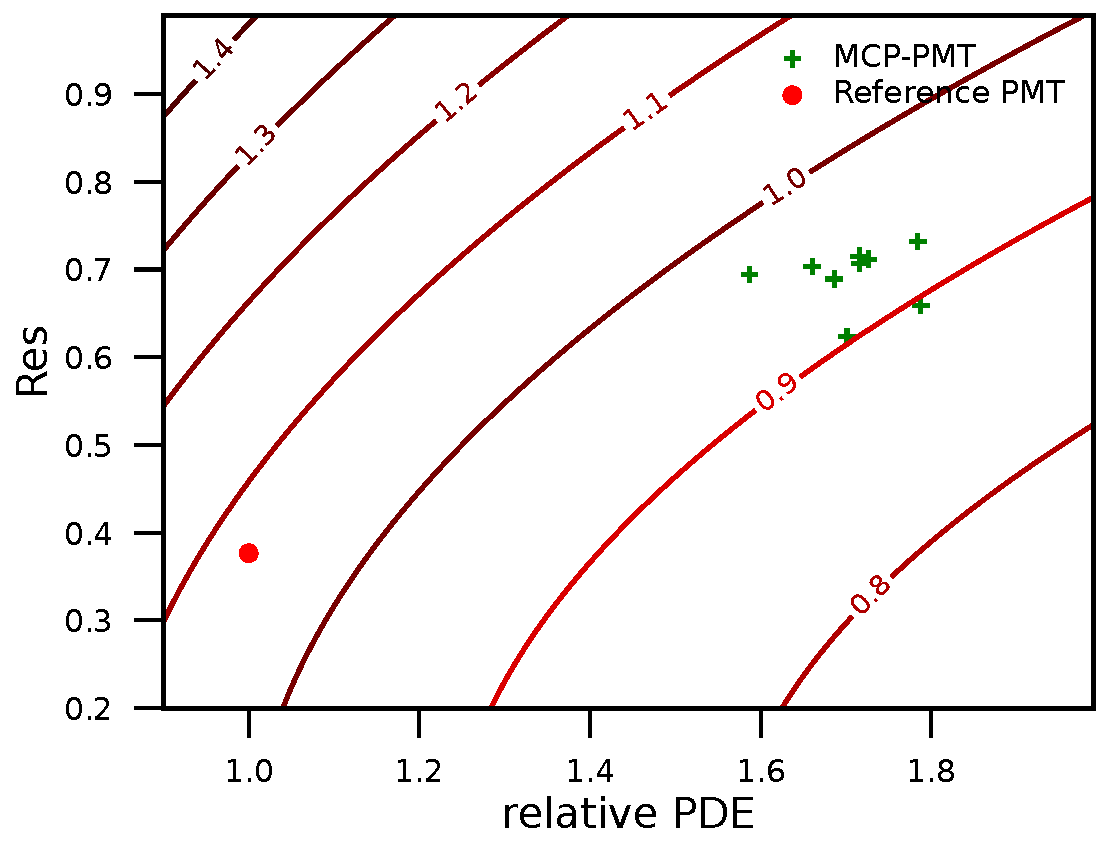
\includegraphics[width=\textwidth]{../figures/result/resolution.pdf}
            \end{figure}
        \end{column}
        \begin{column}{0.6\textwidth}
            \begin{itemize}
                \item the number of expected photons $N$ on a PMT: $\pi(\mu_N)$
                \item Energy $E$ of an event is proportional to $N=k\eta E$
                \item The output charge distribution $C$ is a hierarchical model
            \end{itemize}
            \begin{align}
                E[C]&=\mu_N\mu_C\\
                Var[C]&=\mu_C^2\mu_N+\mu_N\sigma_C^2
            \end{align}
        \end{column}
    \end{columns}
 $N$ is estimated as $\hat{N}=\frac{C}{\mu_C}$ and $E$ is estimated as $\hat{E}=\frac{\hat{N}}{k}$. The reconstructed energy resolution
    \[
        \frac{\sqrt{Var[\hat{E}]}}{E[\hat{E}]}=\frac{\sqrt{\mu_c^2\mu_N+\mu_N\sigma_c^2}}{\mu_N\mu_c}=\frac{\sqrt{1+(\frac{\sigma_c}{\mu_c})^2}}{\sqrt{\mu_N}}=\frac{\sqrt{1+(\frac{\sigma_c}{\mu_c})^2}}{\sqrt{k\eta E}}
    \]
\end{frame}
\section{Summary}
\begin{frame}{Summary}
    \begin{itemize}
    \item The expected relative PDE of the new type 8-inch MCP-PMT is significantly high and is about 1.7 times higher than the reference PMT. 
    \item Although the resolution of the total charge is worse, the ability for boosting energy resolution is promising.
    \end{itemize}
\end{frame}
\end{document}